\documentclass[12pt]{article}

% --- Página y tipografía ---
\usepackage[letterpaper,margin=2.5cm]{geometry}
\usepackage[T1]{fontenc}
\usepackage[utf8]{inputenc} % si compilas con pdfLaTeX
\usepackage{lmodern}
\usepackage{microtype}

% --- Imágenes y color ---
\usepackage{graphicx}
\usepackage{xcolor}

% --- Control fino de espacios ---
\usepackage{setspace}
\setlength{\parindent}{0pt}

\begin{document}
\thispagestyle{empty}

% ===== Encabezado con logos + texto =====
\begin{minipage}[c]{0.18\textwidth}
    \centering
    % Cambia por tu logo izquierdo
    % \includegraphics[width=0.95\linewidth]{img/logo_usac.jpeg}
\end{minipage}
\hfill
\begin{minipage}[c]{0.60\textwidth}
    \small
    Universidad de San Carlos de Guatemala\\
    Escuela de Ciencias Físicas y Matemáticas\\
    Nombre estudiante Diego Andre Torres Castañeda\\
    Carnet: 2026046 \\
    Programación 1\\
\end{minipage}
\hfill
\begin{minipage}[c]{0.18\textwidth}
    \centering
    % Cambia por tu logo derecho
    
\includegraphics[width=1.4\linewidth]{logo1_0.jpg}
\end{minipage}

\vspace{0.5cm}

% Línea horizontal superior (gruesa)
\noindent\rule{\textwidth}{1.2pt}

\vspace{0.2cm}

% ===== Título =====
\begin{center}
    {\Large\scshape Ensayo}\\[0.3em]
\end{center}

\vspace{0.1cm}

% Fecha
\begin{center}
    \small\scshape 06 de febrero de 2026
\end{center}

\vspace{0.2cm}

% Línea horizontal inferior (gruesa)
\noindent\rule{\textwidth}{1.2pt}

\vspace{0.6cm}

% ===== Caja de resumen =====
\noindent
\colorbox{gray!35}{%
    \parbox{\textwidth}{%
        \vspace{0.6em}
        \textbf{\textit{Resumen}. Para el lector: Este ensayo trata sobre las futuras aplicaciones en el campo de mi interés, en el cual realizaré investigaciones.} \\[0.3em]
        \small

        \vspace{0.8em}
    }%
}


\section{Objetivos}
\begin{enumerate}
  \item Hacer simulaciones de choques entre particulas sub-atómicas.
  \item Realizar un software que me ayude con las simulaciones.
  \item Trasladarlo a un paper donde se expliquen las investigaciones.
\end{enumerate}
\section{Marco Teórico}
\begin{enumerate}
  \item Se enfocará precisamente en la rama de mecanica cuantica, teoría cuantica de campos, emtre otras.
  \item Se harán las simulaciones em un software hecho en python.
  \item Se crearan gráficas con nuestros resultados.
\end{enumerate}
\section{Diseño Experimental}
Ácá quiero recalcar, aparte de experimentar en programación la fusión y fisión nulcear. La interacción de las partículas, creación de partículas virtuales en espacios computacionales.
Tambien realizar experimentaciones en simulaciones de sistemas dínamicos. Adjunto fotos representativas. 
\begin{figure}[h]
  \centering
  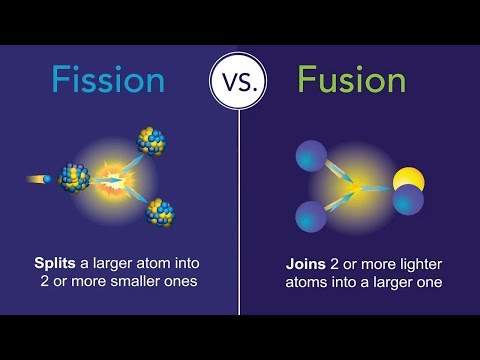
\includegraphics[width=0.3\textwidth]{hqdefault.jpg}
\end{figure}
\begin{figure}[h]
  \centering
  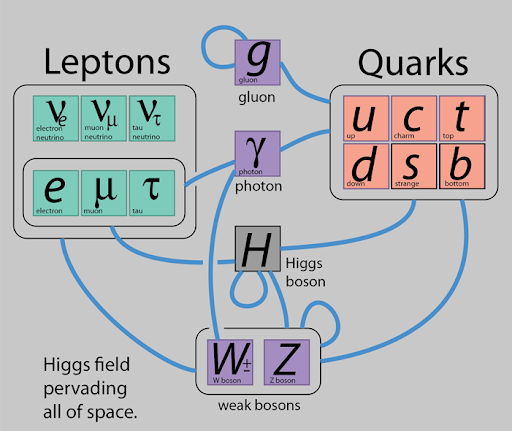
\includegraphics[width=0.3\textwidth]{Particles.png}
\end{figure}
\section{Resultados}
Espero tener resultados que coincidan con los demás estudios hechos o asimilarlos, comprobar hasta que elementos se cumple la fusión o la fisión. Probar todos los resultados de los sistemás dinamicos.
\section{Discusión de Resultados}
Se evaluaron los resultados con los demás estudios publicados en el campo. Se llega a una conclusión en base a los patrones que nos proporcionan las simulaciones.
\section{Conclusiones}
Al ya haber realizado completamente un número considerable de simulaciones de la fisión y fusión se traen los resultados obtenidos sobre los procesos que realizan las particulas al momento de fusionarse o hacer fisión.
\section{Referencias}

\section{Anexos}
\end{document}

\end{document}